%% Простая презентация с примером включения программного кода и
%% пошаговых спецэффектов
\documentclass{beamer}
\usepackage{fontspec}
\usepackage{xunicode}
\usepackage{xltxtra}
\usepackage{xecyr}
\usepackage{hyperref}
\setmainfont[Mapping=tex-text]{DejaVu Serif}
\setsansfont[Mapping=tex-text]{DejaVu Sans}
\setmonofont[Mapping=tex-text]{DejaVu Sans Mono}
\usepackage{polyglossia}
\setdefaultlanguage{russian}
\usepackage{graphicx}
\usepackage{listings}
\lstdefinestyle{mycode}{
  belowcaptionskip=1\baselineskip,
  breaklines=true,
  xleftmargin=\parindent,
  showstringspaces=false,
  basicstyle=\footnotesize\ttfamily,
  keywordstyle=\bfseries,
  commentstyle=\itshape\color{gray!40!black},
  stringstyle=\color{red},
  numbers=left,
  numbersep=5pt,
  numberstyle=\tiny\color{gray},
}
\lstset{escapechar=@,style=mycode}
\usepackage{graphicx}       % работа с картинками
\usepackage{float}          % необходимо для указания места картинки на странице
\usepackage[export]{adjustbox}  % еще про место картинки (width,right/left])

\usepackage{multirow} % для няшных табличек       

\begin{document}
    \title{Рекомендательная система для образовательного контента}
    \author{Лена Волжина\\{\footnotesize\textcolor{gray}{куратор: Николай Вяххи}}}
    \institute{СПбГУ}
    \date{24 декабря 2015 г.}     % можно поставить какую-нибудь дату
\frame{\titlepage}

\begin{frame}\frametitle{Введение} 
    \begin{itemize}
        \item онлайн-образование
        
        \begin{table}[H]
            \caption{Платформы с онлайн-курсами}
            \label{tabular:statistic}
            \begin{center}
            \begin{tabular}{c|c|c}
            \hline
            Название & Год запуска & Пользователей \\
            \hline
            Coursera & 2012 & 15 млн \\
            edX & 2012 & 5 млн \\
            Udacity & 2012 & 1.6 млн \\
            Stepic.org & 2013 & 130 тыс. \\
            
            \end{tabular}
            \end{center}
        \end{table}
    
        \item плюсы: доступность, масштабируемость % индивидуальный график
        \item минусы: отсутствие программы обучения, индивидуального подхода
        % кажется естественным применять рекомендательные системы
    \end{itemize}
\end{frame}



\begin{frame}\frametitle{Рекомендательные системы} 
    
    Классификация\cite{rec_sys_handbook}:
    \begin{itemize}
    	\item фильтрация контента
    	\item коллаборативная фильтрация    % использует известные оценки для предсказания неизвестных
    \end{itemize}
    % есть и другие, более специфичные задачам
    
    \bigskip
    
    Оценка результатов\cite{rec_sys_handbook:evaluation}:   % аспекты для оценивания
    \begin{itemize}
    	\item точность предсказаний     % полезно, когда нужно предсказать оценку, считаем отклонение реального от предсказанного
    	\item предсказание потребности  % когда нет явных оценок. примеры: точность, полнота, основанные на них метрики
    	\item адаптивность      % особенно важно для образовательного контента
    	\item новизна, доверие пользователя, разнообразность и прочие
    \end{itemize}
    % метрики позволяют оценить систему или скорее сравнить разные ее версии
\end{frame}



\begin{frame}\frametitle{Постановка задачи}
Платформа stepic.org
    \begin{itemize}
    	\item онлайн-курсы и библиотека уроков
    	\item русскоязычный ресурс, техническая тематика
    \end{itemize}

\bigskip

\begin{figure}[H]
    \center{
\includegraphics[width=0.7\linewidth]{images/stepic_youtube.PNG}}
\end{figure}
    
% гибридная рекомендательная система со свойством адаптивности
% оценка вышеупомянутыми метриками

\end{frame}



\begin{frame}\frametitle{Текущие результаты}
    
    \begin{figure}[H]
        \center{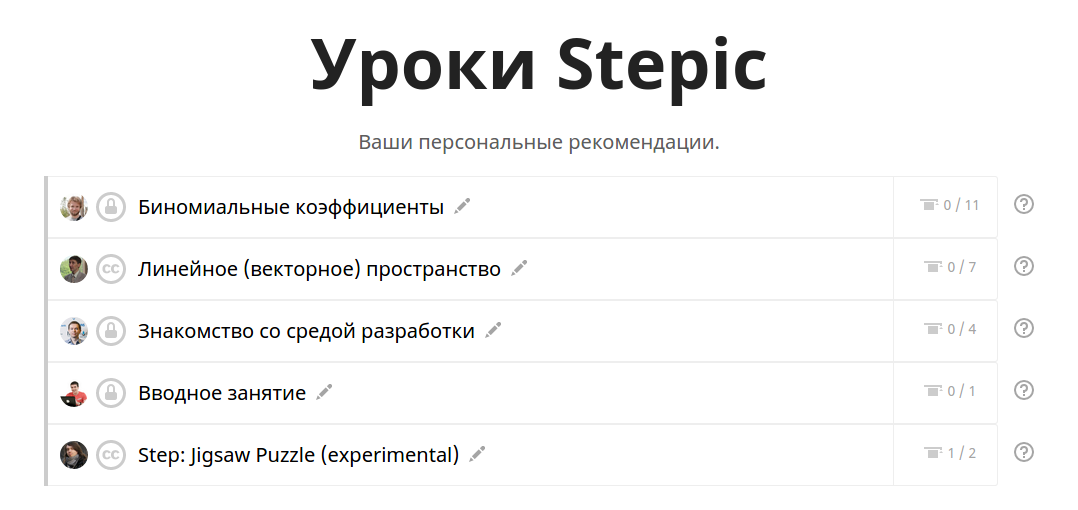
\includegraphics[width=\linewidth]{images/rec.png}}
    \end{figure} 
    
    % смесь фильтрации контента по языкам, тегам, сложности и коллаборативной фильтрации
\end{frame}



\begin{frame}\frametitle{Текущие результаты}
    
    \begin{figure}[H]
        \center{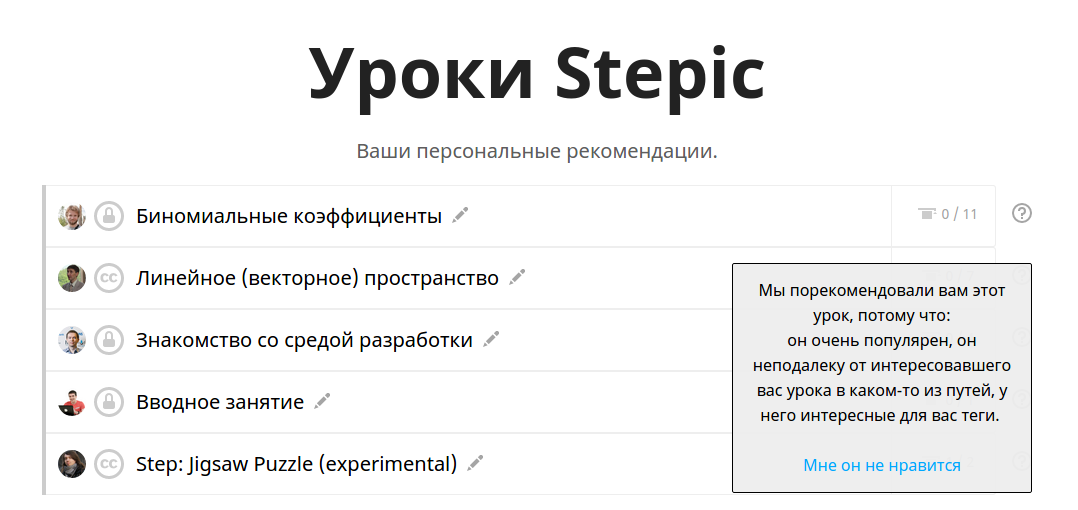
\includegraphics[width=\linewidth]{images/rec_expl.png}}
    \end{figure} 
    
    % объяснения добавляют доверия, отказы пока плохо работают
\end{frame}


\begin{frame}\frametitle{Планы: адаптивность}
Пример: knewton.com\cite{knewton_paper}
    \begin{itemize}
    	\item дифференцированное обучение       % предустановленные пути
    	\item персонализированное обучение      % индивидуальный путь для студента, основанный обычно на правилах с деревом решений 
    	\item адаптивное обучение  (\textit{data-driven education})      % постоянно совершенствуется для каждого студента, основываясь на новых данных,  в отличие от стандартной оценки "в одной точке"
    \end{itemize}
    
    \begin{figure}[H]
        \center{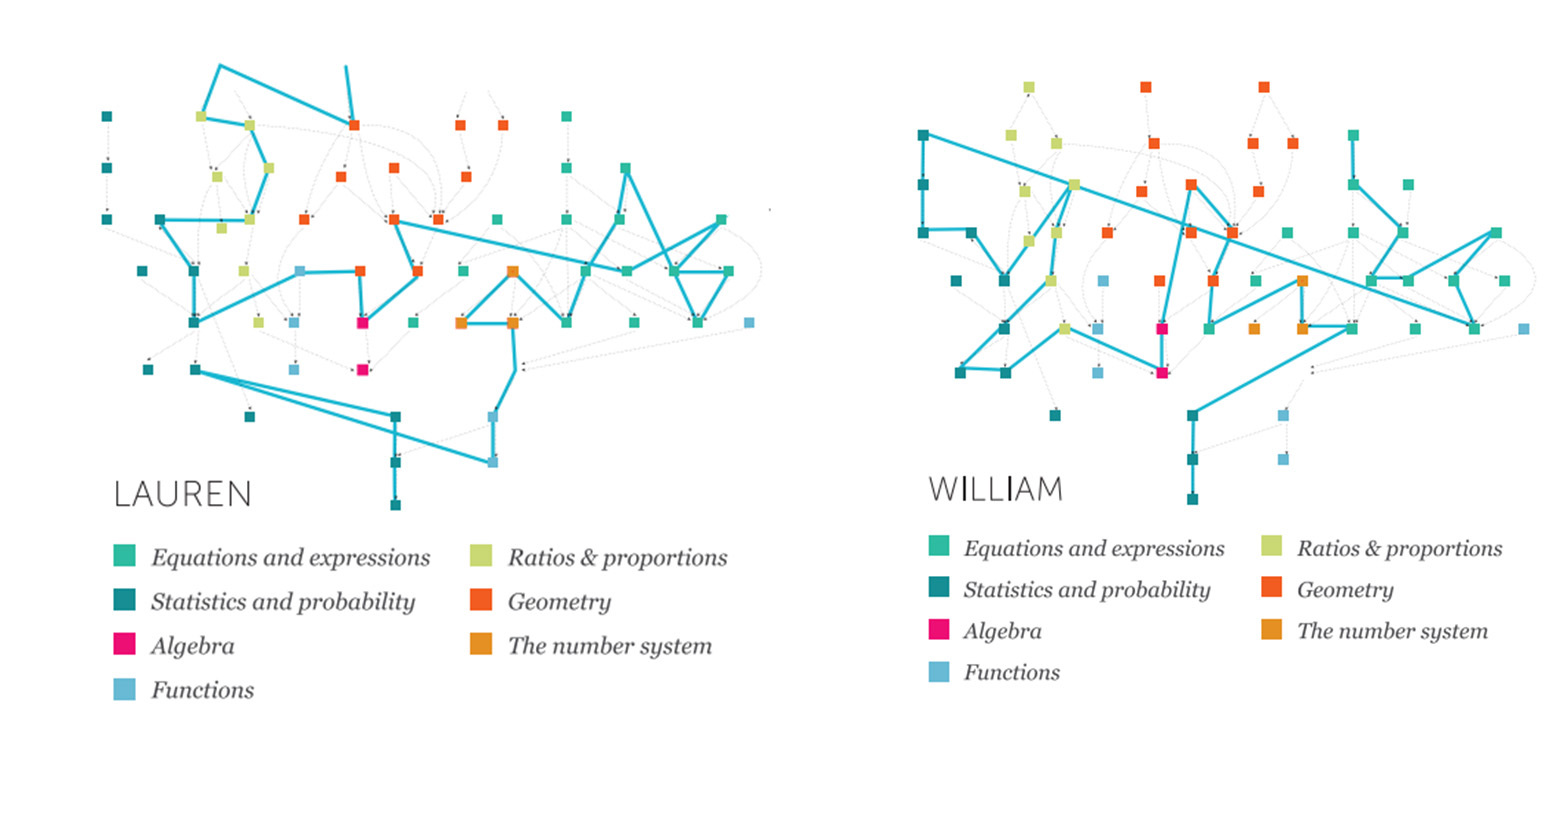
\includegraphics[width=0.8\linewidth]{images/knewton.jpg}}
    \end{figure} 
\end{frame}


\begin{frame}\frametitle{Литература}
\setmonofont[Mapping=tex-text]{CMU Typewriter Text}
\bibliographystyle{ugost2008ls}
\bibliography{diploma.bib}
\end{frame}


\begin{frame}
\huge{Спасибо! \\\indent \\\indent Вопросы?}
\end{frame}


\end{document}